\documentclass[conference]{IEEEtran}


\usepackage{cite}
\usepackage{amsmath,amssymb,amsfonts}
\usepackage{algorithmic}
\usepackage{graphicx}
\usepackage{textcomp}
\usepackage{xcolor}
\def\BibTeX{{\rm B\kern-.05em{\sc i\kern-.025em b}\kern-.08em
    T\kern-.1667em\lower.7ex\hbox{E}\kern-.125emX}}

\begin{document}
\title{Exploring the Bayes Classifier: A Deep Dive into Linearly Separable Data with Diagonal Covariance\\
\thanks{Identify applicable funding agency here. If none, delete this.}
}

\author{\IEEEauthorblockN{Pawan Ram Mali(PhD)}
\IEEEauthorblockA{\textit{Department of CSE } \\
\textit{Indian Institute Of Technology}\\
Dharwad, India \\
cs24dp011@iitdh.ac.in}
\and
\IEEEauthorblockN{Sachin Maurya (MS)}
\IEEEauthorblockA{\textit{Department of CSE} \\
\textit{Indian Institute Of Technology}\\
Dharwad, Indian \\
cs24ms002@iitdh.ac.in}
\and
\IEEEauthorblockN{Abhishek Sharma (MS)}
\IEEEauthorblockA{\textit{Department of CSE} \\
\textit{Indian Institute of Technology}\\
Dharwad, India \\
cs24ms003@iitdh.ac.in}
}

\maketitle

\begin{abstract}
\\
The Bayes classifier is a key technique in statistical pattern recognition, and this project delves into both its theoretical basis and practical application. The task involves classifying objects with two-dimensional features into one of three distinct categories, with each class's data stored in separate text files. The goal is to create a classifier capable of accurately predicting the class of new, unseen data.

The project begins with exploratory data analysis (EDA), using visual tools to inspect the data’s distribution, detect any class overlap, and identify potential outliers. Following EDA, we prepare the data by splitting it into training and testing sets to assess the classifier’s performance, and apply feature scaling to ensure consistency.

A critical aspect of this project is validating the assumptions underlying the Bayes classifier. As the Bayes classifier performs best under the assumption of Gaussian-distributed features, we verify this condition for each class. Additionally, we calculate class priors to address any imbalances in the dataset and investigate the independence of features, which is especially important for the Naive Bayes variant.

The core of the project involves applying the Bayes classifier. We estimate the probability that each data point belongs to a given class using the multivariate Gaussian probability density function, combining these with prior probabilities to assign each data point to the class with the highest posterior probability.

Finally, through testing and visualizing decision boundaries, we evaluate the classifier's effectiveness in separating the feature space. The results demonstrate the Bayes classifier’s capability to accurately distinguish between the three classes, highlighting its potential as a powerful tool in pattern recognition. This project offers hands-on experience in building and assessing a machine learning model from the ground up, while reinforcing the theoretical concepts behind the Bayes classifier.
\end{abstract}

\section{Introduction}
In this project, we explore the application of the Bayes classifier in a pattern recognition problem. Our objective is to classify data points into one of three distinct classes based on their features. The dataset consists of three classes, each represented by a set of two features, which likely correspond to measurements or observations in a specific domain. The Bayes classifier will be implemented to predict the class membership of new, unseen data points.

It focuses on classifying data points into three distinct classes by calculating the posterior probability using Bayes' theorem. The classifier is then evaluated using various metrics, and its decision boundaries are visualized through a series of plots.
 
	\[
	P(C_k \mid x) = \frac{P(x \mid C_k) \cdot P(C_k)}{P(x)}
	\]
	
	\begin{itemize}
		\item \textbf{Posterior Probability} \( P(C_k \mid x) \): The probability of the class \( C_k \) given the observed data \( x \). It represents the updated belief after considering the evidence (data).
		
		\item \textbf{Prior Probability} \( P(C_k) \): The probability of the class \( C_k \) before observing the data \( x \). It reflects the initial belief about the class.
		
		\item \textbf{Likelihood} \( P(x \mid C_k) \): The probability of the observed data \( x \) given that the class is \( C_k \). It measures how likely the data is for each class.
		
		\item \textbf{Evidence} \( P(x) \): The total probability of observing the data \( x \) under all possible classes. It acts as a normalizing constant and ensures that the posterior probabilities sum to 1.
	\end{itemize}


\section{Objectives}

The key objectives of this project are:

\begin{enumerate}
	\item \textbf{Classifier Development:} Build a Bayesian classifier based on multivariate Gaussian distributions for three classes of data.
	\item \textbf{Model Evaluation:} Use statistical metrics such as confusion matrix, accuracy, precision, recall, and F1-score to evaluate the classifier’s performance.
	\item \textbf{Decision Boundary Visualization:} Visualize the decision boundaries that separate the different classes, allowing for a clear understanding of how the classifier behaves.
\end{enumerate}


\section{Exploratory Data Analysis(EDA) }
Before implementing the classifier, it is essential to explore and understand the data.
Loading and Visualizing the Data We start by loading the data from the text files and visualizing it to gain insights into the distributions and separability of the classes.

\section{Observation }

\subsection{Data Distribution :}
The scatter plot allows us to observe how each class is distributed in the feature space, helping to identify any overlaps or separability between the classes.

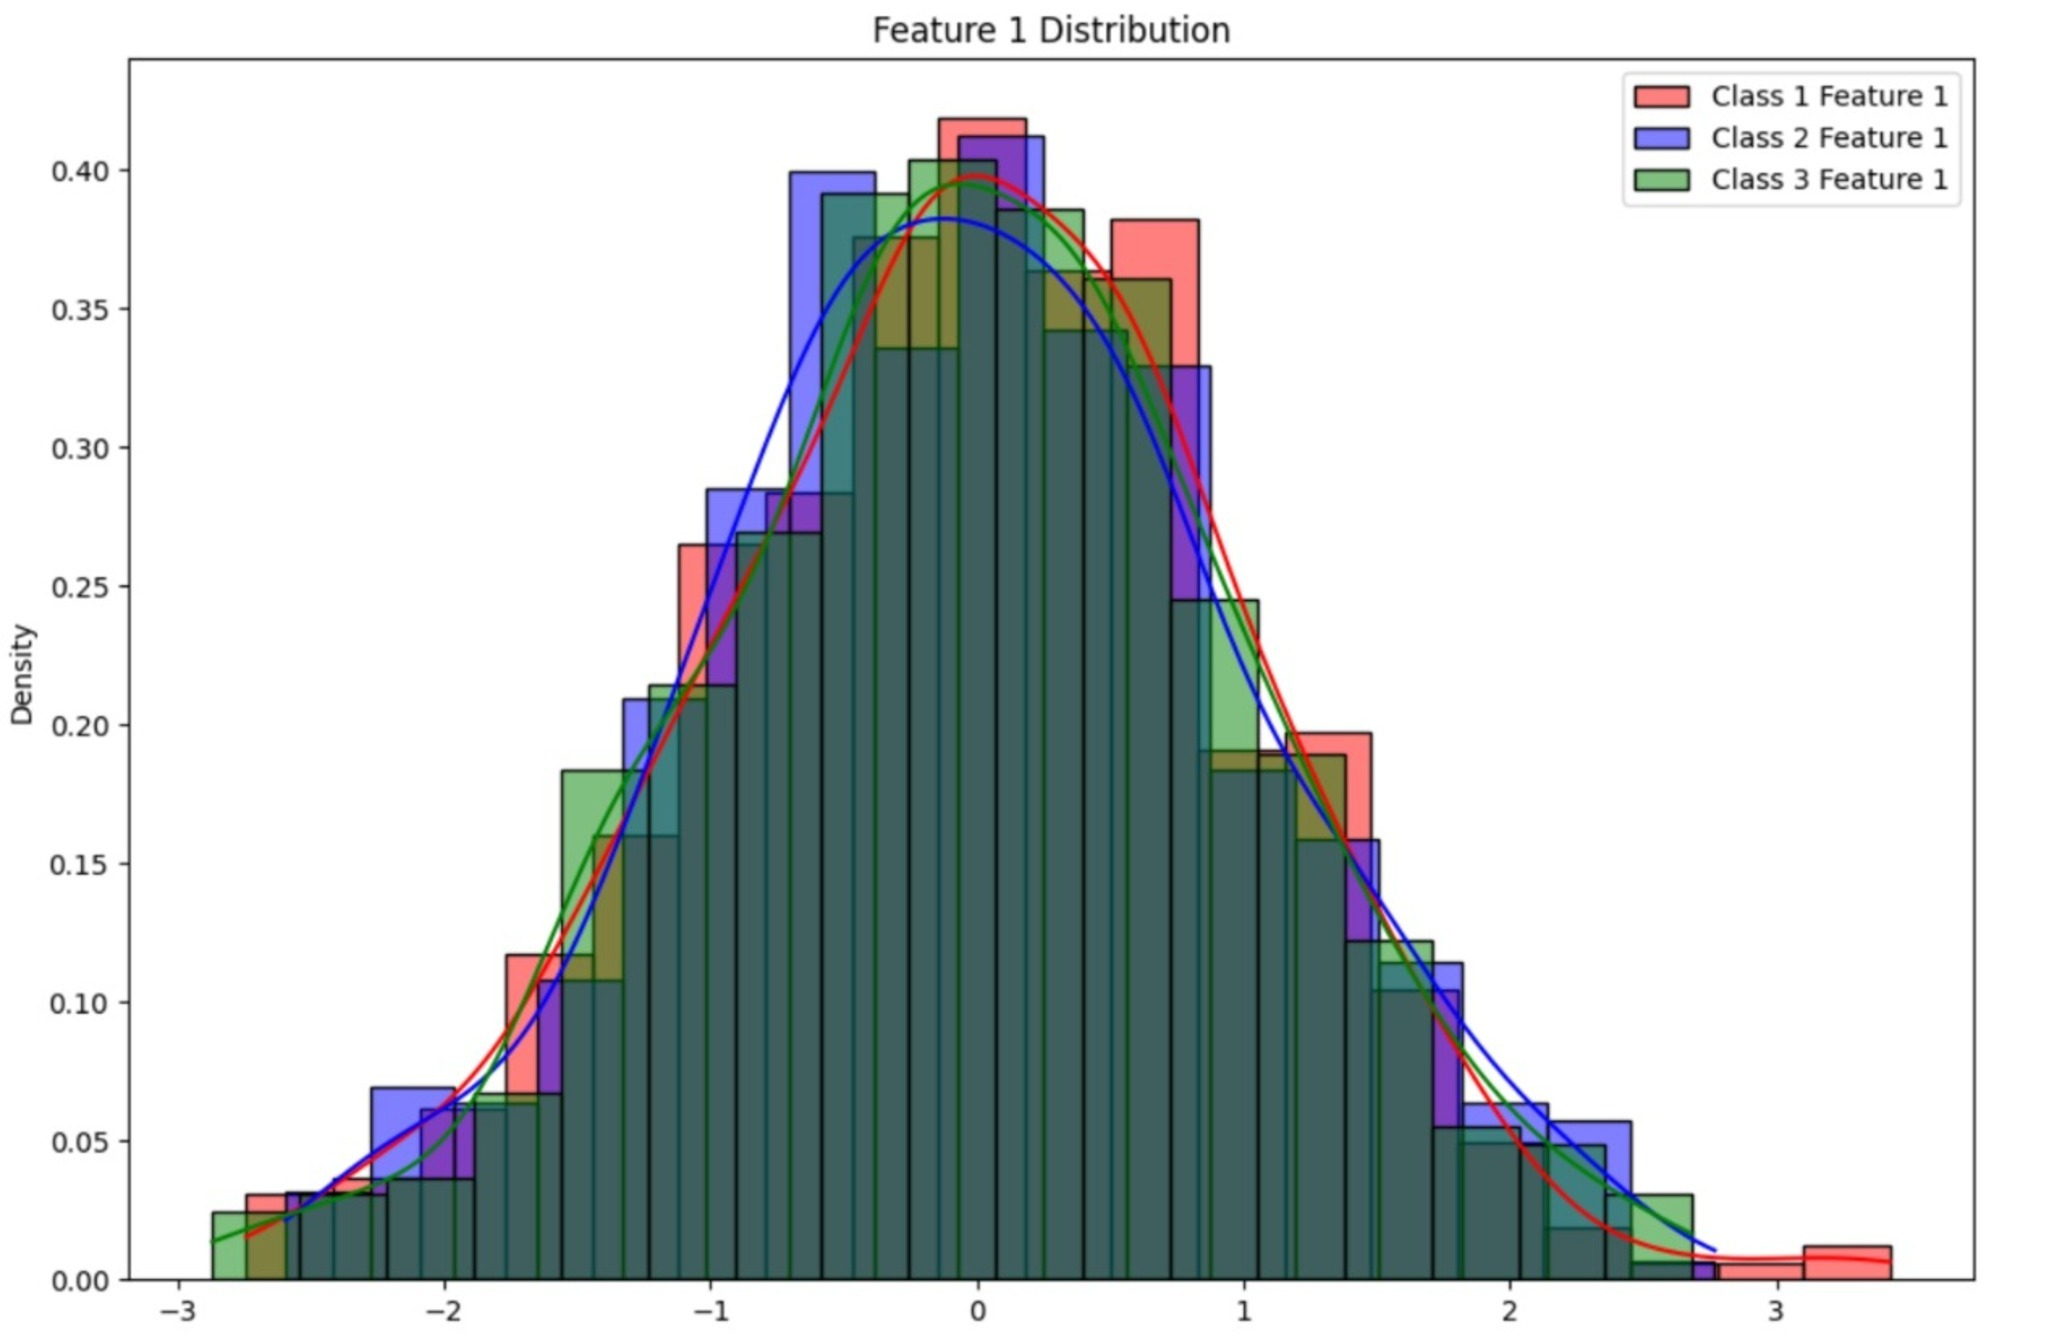
\includegraphics[width=0.5\textwidth, height=5cm]{figr1.jpg}

\subsection{Cluster Formation :}\label{AA}
The plot also reveals any natural clusters within the data that correspond to the different classes.

\section{Data Processing }
To ensure that the data is in a suitable form for the Bayes classifier, we preprocess it accordingly.
\subsection{Steps In Data Processing }
\begin{itemize}
\item Normalization/Standardization: We standardize the data to have zero mean and unit variance.
\item 2.	Handling Missing Data: Although not present in this dataset, missing data would be handled by imputation or removal.
\item Data Splitting: We split the data into training and testing sets to evaluate the classifier's performance.
\end{itemize}

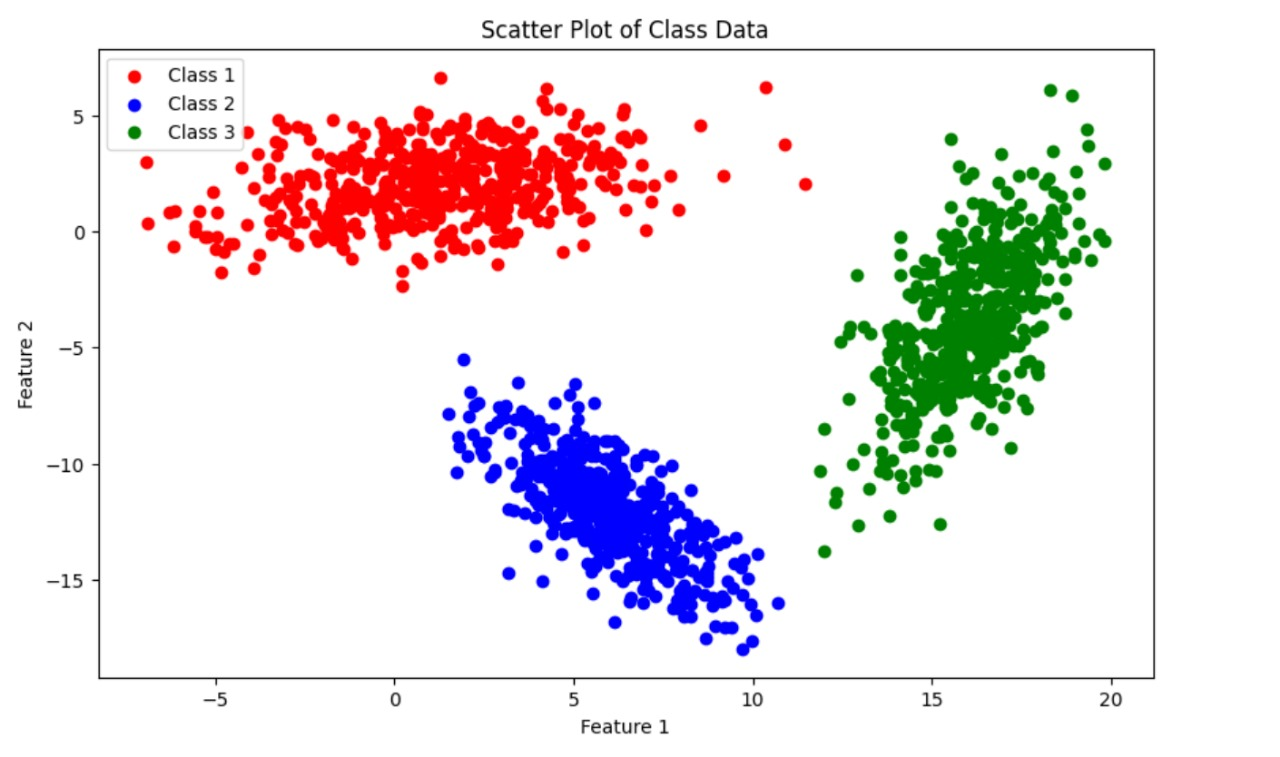
\includegraphics[width=0.5\textwidth, height=5cm]{figr2.jpg}

\subsection{Equations}
Here's the mathematical expression for the Gaussian probability density function (PDF) :
	
	\[
	f(x; \mu, \sigma^2) = \frac{1}{\sqrt{2 \pi \sigma^2}} \exp\left(-\frac{(x - \mu)^2}{2 \sigma^2}\right)
	\]
	
	where:
	\begin{itemize}
		\item \( x \) is the variable,
		\item \( \mu \) is the mean,
		\item \( \sigma^2 \) is the variance,
		\item \( \exp \) represents the exponential function.
	\end{itemize}
	
\subsection{Check Assumptions of the Bayes Classifier}
Before implementing the Bayes classifier, we verify that its assumptions are met.

\subsection{Gaussian Distribution of Features}
The Bayes classifier assumes that the features follow a Gaussian (normal) distribution within each class. We check this assumption by plotting histograms of the features for each class.

\section{Observation}
The histograms indicate whether the feature distributions approximate a normal distribution. If deviations from normality are observed, data transformations may be considered.

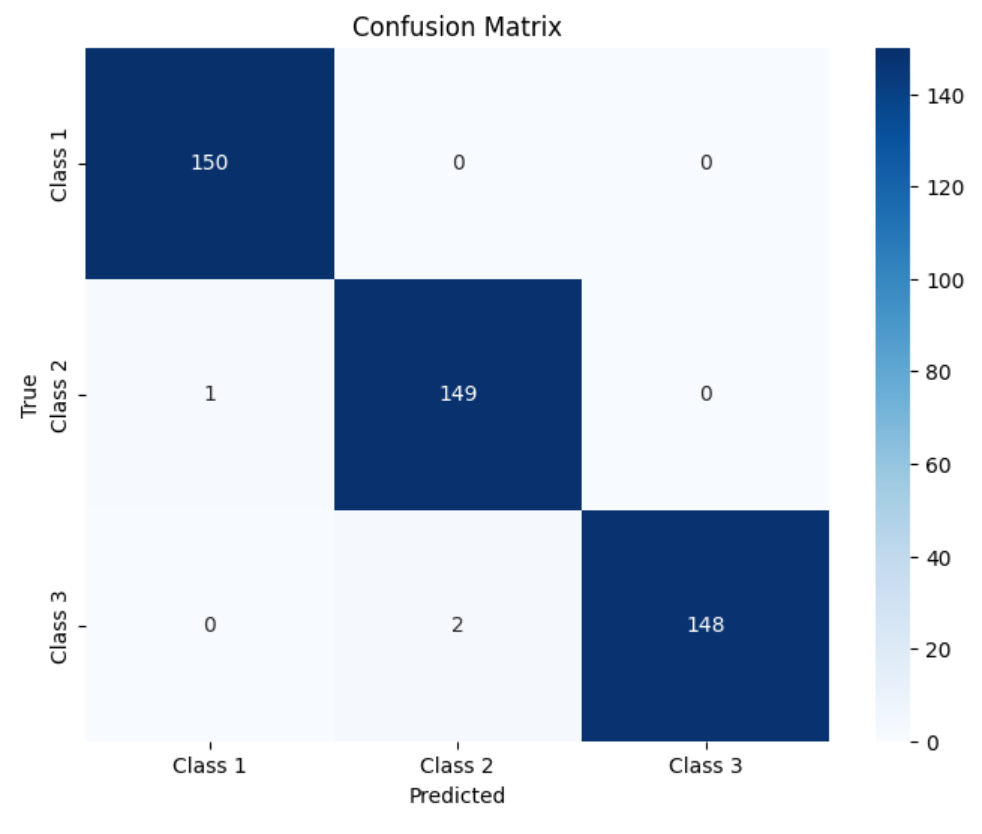
\includegraphics[width=0.5\textwidth, height=5cm]{figr3.png}

\subsection{Class Independence (for Naive Bayes)}\label{CI}
If implementing a Naive Bayes classifier, the features are assumed to be conditionally independent given the class. We can examine the correlations between features within each class to verify this assumption.

\subsection{Class Priors}\label{CP}
We estimate the prior probabilities of each class based on the training data. This step ensures that the classifier accounts for any class imbalances.

\section*{Acknowledgment}

The 


\begin{thebibliography}{00}
\bibitem{b1} G. Eason, B. Noble, and I. N. Sneddon, ``On certain integrals of Lipschitz-Hankel type involving products of Bessel functions,'' Phil. Trans. Roy. Soc. London, vol. A247, pp. 529--551, April 1955.

\end{thebibliography}



\end{document}
